\subsection{Domain Definition}
\label{sub:dmDefine}
Domain is a set of applications, which share common functions and common patterns \newtext{(functions and their connections)}~\cite{kang1990feature}. To allow reasoning about the domain\footnote{Defining the scope of a domain, i.e. assessing domain membership, is an additional research topic.}, we formally define it as a set of graphs.
%Current definitions of domain include a set of applications which share a set of common capabilities and data \cite{kang1990feature}, a class of applications, with a component library, which contains reusable chunks of domain expertise \cite{tracz1995dssa}. Following this definition, we define a domain as a set of applications, which share common functions and common patterns. To allow reasoning about the domain\footnote{Defining the scope of a domain, i.e. assessing domain membership, is an additional research topic.}, we formally define it as a set of graphs.
%\vspace{-5pt}
\begin{equation}
\begin{split}
\label{eq:domain}
	&G = \{g_{0}, g_{1}, ..., g_{N}\}, \quad g_{i} = (A, E)\\
	&A = \{a_{0}, a_{1}, ..., a_{n}\}, \quad E = \{e_{0}, e_{1}, ..., e_{m}\}\\
	&a_{i} (t, d_{P}), \quad e_{i} ((a_{src}, a_{dst}), d_{C})
\end{split}
\end{equation}
%\endgroup
%\vspace{-10pt}

In Eq.~\eqref{eq:domain}, domain $G$ is a set of streaming applications ($g_{0}$ .. $g_{N}$), each captured as a dataflow graph \cite{stuijk2006sdf}. Each application $g_i$ contains a set $A$ of processing actors ($a_0$ .. $a_n$) and a set of $E$ edges ($e_0$ .. $e_m$) representing the communication between actors. Each actor $a_i$ is an instance of a function type $t$ with an instance-specific processing demand $d_{P}$ (\# of operations). Multiple instances of the same function type $t$ may exist within and across applications within the domain. Each edge $e_i$ is the directed communication between its \newtext{source actor} $a_{src}$ and \newtext{destination actor} $a_{dst}$ with a communication demand of $d_{C}$ as a measure of the transferred volume (bytes). E.g., in application $g0$ of Fig.~\ref{fig:Apps}, the first actor $A0$ is an instance of $t_{A}$ and its $d_{P} = 350$, and the edge between $A0$ and $B0$ contains $d_{C} = 50$. 

\begin{table}[h]
  \begin{minipage}[b]{0.35\linewidth}
    \centering
    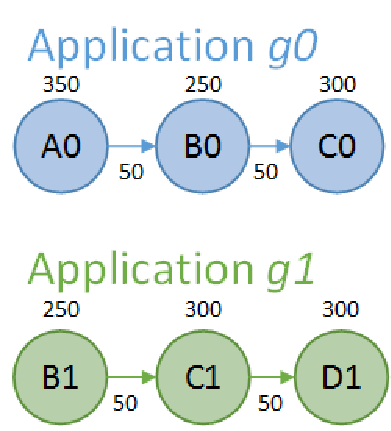
\includegraphics[width=0.9\linewidth]{fig/Apps.pdf}
    \captionof{figure}{Example: Domain Applications}
    \label{fig:Apps}
  \end{minipage}
	 \hfill
  \begin{varwidth}[b]{0.6\linewidth}
    \centering
    \begin{tabular}{l r r r}
      \toprule
      Composition & $P$ & $D_{P}$ & $D_{C}$ \\
      \midrule
      $\{t_A\}$ & 50\% & 350 & -- \\
      $\{t_B\}$ & 100\% & 500 & -- \\
      $\{t_C\}$ & 100\% & 600 & -- \\
      $\{t_D\}$ & 50\% & 300 & -- \\
			\hline
			$\{t_A,t_B\}$ & 50\% & -- & 50 \\
			$\{t_B,t_C\}$ & 100\% & -- & 100 \\
			$\{t_C,t_D\}$ & 50\% & -- & 50 \\
			\hline
			$\{t_A,t_B,t_C\}$ & 50\% & -- & -- \\
			$\{t_B,t_C,t_D\}$ & 50\% & -- & -- \\			
      \bottomrule
    \end{tabular}
    \caption{Example: Domain Features}
    \label{tab:egFeature}
  \end{varwidth}
\end{table}